\pdfoutput=1 
\documentclass[12pt,a4paper]{article}
\usepackage{cite}
\usepackage{calligra}

\usepackage{xcolor}
\definecolor{darkPurple}{HTML}{3333B2}
\definecolor{forestGreen}{HTML}{337700}
\definecolor{shadecolor}{HTML}{CCCCCC}
\definecolor{darkGrey}{HTML}{4E4F86}
\definecolor{Crimson}{HTML}{DC143C}
\definecolor{transparentBlue}{HTML}{EBEBF8}
\usepackage{hyperref}
\hypersetup{colorlinks=true, linkcolor=darkPurple, citecolor=darkPurple}
\usepackage[pdftex]{graphicx}
\graphicspath{{./figures/}}
\usepackage[cmex10]{amsmath}
\usepackage{amssymb}
\usepackage{multirow}	
\usepackage[]{subfig}
\usepackage[toc]{appendix}
\usepackage{listings}
\usepackage[english]{babel}
\lstset { %
  language=C,
  backgroundcolor=\color{black!5}, % set backgroundcolor
  basicstyle=\footnotesize,        % the size of the fonts that are used for the code
  commentstyle=\color{forestGreen},    % comment style
  keywordstyle=\color{blue},       % keyword style
  keepspaces=true,                 % keeps spaces in text, useful for keeping indentation of code (possibly needs columns=flexible)
  showspaces=false,
  showstringspaces=false
}
% Font settings to get IEEE-style fonts
\renewcommand{\sfdefault}{phv}
\renewcommand{\rmdefault}{ptm}
\renewcommand{\ttdefault}{pcr}

\title{{\Huge Sitar}\\
{\large Simulation Tool for Architectural Research}\\[1em]
User's Manual}

\author{Neha V. Karanjkar \qquad Madhav P. Desai\\
{\small Department of Electrical Engineering}\\
{\small Indian Institute of Technology Bombay}\\[1em]

\includegraphics[width=0.15\textwidth]{./figures/iitblogo.pdf}\\
}
\date{}
\begin{document}
\maketitle

\begin{abstract}
Sitar is a tool for modeling and simulation of cycle-based systems.
It consists of a system description language and a simulation kernel.  
%
A system in sitar can be described as a set of interconnected modules running
concurrently on a single clock.  The language supports hierarchical
descriptions: modules can contain instances of other modules.
%
The behavior of each module can be described in an imperative manner as a
sequence of statements.  The statements include constructs such as time delays,
parallel blocks, branch/loop constructs, procedures and
instantaneous code blocks.  C++ code can be embedded in a module description at
several places in a straightforward and well defined manner.
Each module description gets translated to a C++ class. The generated code can
be compiled and linked together with the simulation kernel to get a single
simulation executable.  
%
The simulation kernel is lightweight, consisting of a
small set of C++ classes, and supports parallel execution using OpenMP. 
The simulation algorithm uses two-phase execution : each clock cycle
is divided into two phases, and input/output events are
restricted to separate phases, leading to a race-free execution.
\end{abstract}
\tableofcontents
\newpage



\section{Basic Components} \label{sec:Components}
A system is composed of {\em modules} and {\em nets}.
Modules represent behavioral entities in the system,
and nets are channels of communication between them.
All modules run concurrently on a single clock.
A module can communicate with another module
by transfer of {\em tokens} (which are packets of
information) over nets.
Nets provide finite-capacity
FIFO buffering for tokens.
%
A module's interface to a net is called 
a {\em port}. A port can either be an {\em inport} or an {\em outport}.
Each net is connected to exactly one inport and one outport.
Figure \ref{fig:ExecutionModel} shows an example of a system 
with three modules.
%
\begin{figure}[h]
\centering
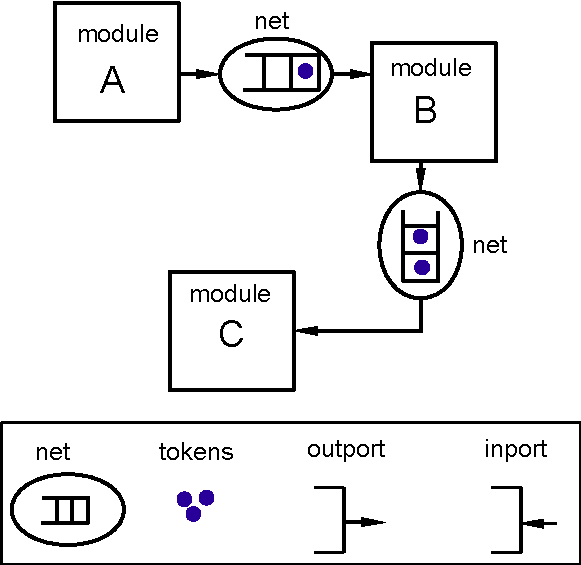
\includegraphics[width=0.6\textwidth]{ExecutionModel.pdf}
\caption{Example of a system in sitar}
\label{fig:ExecutionModel}
\end{figure}

\begin{itemize}
\item Tokens have a {\tt width} parameter, which represents the
number of bytes of data that are carried by the token.

\item A net has two parameters:
{\tt width} and {\tt capacity}. A net with width $W$ can only 
contain tokens of width $W$. The capacity of a net is the maximum number
of tokens it can contain at a time.

\item Ports have a single parameter {\tt width}. A port with width $W$ can only be 
connected to a net of width $W$.
\end{itemize}

\section{The Execution Model}\label{sec:ExecutionModel}
Sitar uses a two-phase execution model.
Each clock cycle is divided into two phases : {\em phase-0}
and {\em phase-1}. A module is allowed to perform input in
phase-0 only, and output in phase-1 only. Thus, reads and writes
to a net can never occur simultaneously and the execution is deterministic.
As a consequence, the propagation of information from one
module to another incurs a delay of at-least one clock cycle\footnote{
The system can thus be viewed as a set of interconnected Moore machines}.
%
This restriction leads to a very simple simulation algorithm
that is easily parallelized. During each phase, 
the behavior of each module in the system is executed exactly once.
The order of execution among modules does not matter.
The simulation algorithm is as follows:

\begin{verbatim}
cycle = 0
while (cycle < total_cycles)
{
   phase=0
   for each module m :
        run m
   phase=1
   for each module m :
        run m
   cycle=cycle+1
}
\end{verbatim}
Within a phase, modules can be executed independently of each other.
Thus the execution of individual modules can be mapped to 
separate threads running in parallel
and synchronizing at the end of each phase.


\section{System Description Language} \label{sec:Language}

\subsection{Basic Design Units}
The basic design units in a sitar description are {\em modules} and {\em procedures}.
Modules represent structural entities in a system. They have a structure as well
as a behavior. Procedures are akin to functions in C. They 
represent a set of actions that can be invoked by modules.
A module or a procedure can be defined once and instantiated multiple times.
Each definition must be contained within a single file. 
However a single file can contain multiple module/procedure definitions.



The system can be described in a hierarchical manner, 
with modules containing instances of
other modules.  The description must always contain a single module named
\lq\lq Top" which represents the top-level module in the structural
hierarchy, and contains all other modules in the system.  
This top-level module is instantiated during simulation.
%
The following is an example of a system 
where the Top module contains two instances 
of a module \lq Foo\rq.
\begin{verbatim}
module Foo
end module

module Top
    submodule f1,f2 : Foo
end module
\end{verbatim}



\end{document}
